\documentclass[a4paper,12pt]{article}
\usepackage[MeX]{polski}
\usepackage[utf8]{inputenc}
\usepackage{graphicx}

%opening
\title{Ringerike}

\author{Adam Stepańczuk}

\begin{document}

\maketitle


Gmina Ringerike (norw. Ringerike kommune) --- norweska gmina leżąca w~regionie Buskerud. Jej siedzibą jest miasto Hønefoss.

Ringerike jest 46. norweską gminą pod względem powierzchni (Rysunek~\ref{zdj1}). 
Położenie na mapie okręgu (Rysunek~\ref{zdj2}).

\begin{table}[here]
\centering
\begin{tabular}{l|l}
Państwo & Norwegia \\
Region & Buskerud \\
Siedziba &  	Hønefoss \\
Kod statystyczny & $0605$ \\
Powierzchnia & 1553,3$^2$ \\
Populacja & \\
liczba ludności & $28 079$ \\
gęstość & $18.08$os./km$^2$ \\

\end{tabular}
\end{table}



\section{Demografia}

Według danych z~roku 2005 gminę zamieszkuje 28 079 osób. Gęstość zaludnienia wynosi 18,08 os./km$^2$. Pod względem zaludnienia Ringerike zajmuje 26. miejsce wśród norweskich gmin.
\newline \newline
ludność
stan na~1~stycznia~2005
\begin{table}[here]
\centering
\begin{tabular}{c|ccc}
 & kobiety & mężczyźni & razem \\
\hline
osób & $13 823$ & $14 256$ & $28 079$ \\
\% & $49.23\%$ & $50.77\%$ & $100\%$ \\
\end{tabular}
\end{table}

wykształcenie
stan na~1~października~2004
\begin{table}[here]
\centering
\begin{tabular}{c|cccc}
 & podst. & średnie & wyższe & niezn. \\
\hline
osób & 5262 & 12 824 & 4260 & 570 \\
\% & $22.96\%$ & $55.96\%$ & $18.59\%$ &  $2.49\%$ \\
\end{tabular}
\end{table}

\section{Edukacja}
Według danych z~1~października~2004:
\begin{itemize}
\item liczba szkół podstawowych (norw. ,,grunnskolar''):~20
\item liczba uczniów szkół podst.:~3538
\end{itemize}

\section{Władze gminy}
Według danych na~rok~2011 administratorem gminy (norw. ,,rådmann'') jest Wenche Grinderud, natomiast burmistrzem (norw.~ordfører, d.~borgermester) jest Kjell Børre Hansen.
\begin{figure}[p]
\caption{}
\label{zdj1}
\centering
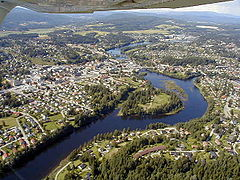
\includegraphics{Ringerike.jpg}
\end{figure}

\begin{figure}[p]
\caption{}
\label{zdj2}
\centering
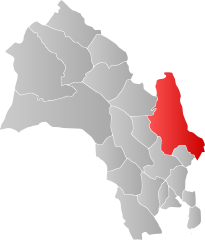
\includegraphics{Mapka.png}
\end{figure}

\begin{thebibliography}{99}
\bibitem{DaneLiczbowe}
\emph {}dane liczbowe: Statistisk sentralbyra
\bibitem{DaneAdresowe}
\emph {}dane adresowe i dotyczące władz: Kommunenøkkelen
\end{thebibliography}

\end{document}